\documentclass[10pt,a4paper]{article}
\usepackage[margin=18mm]{geometry}
\usepackage{amsmath,amssymb,graphicx,booktabs,hyperref}
\hypersetup{colorlinks=true,urlcolor=blue}
\setlength{\parindent}{0pt}
\setlength{\parskip}{5pt}
\raggedright
\begin{document}
\begin{center}
{\Large Aligned auxiliary P-256 factor base}\\
2026-11-14 --- native construction and prospective solver comparison
\end{center}

Actual registered P-256 is used throughout. The development fixture
\texttt{FB1h2704fe49495e} has nine columns and eighteen signed points.
Its structured presentations have maximum input degree 3 versus
same-base dense degree 9. \textbf{Regularity and speedup are unmeasured.}
These observations are unsigned producer evidence [pcc:unverified],
claim \texttt{PCC-20261114-4a3ab6}, without a signed verdict.

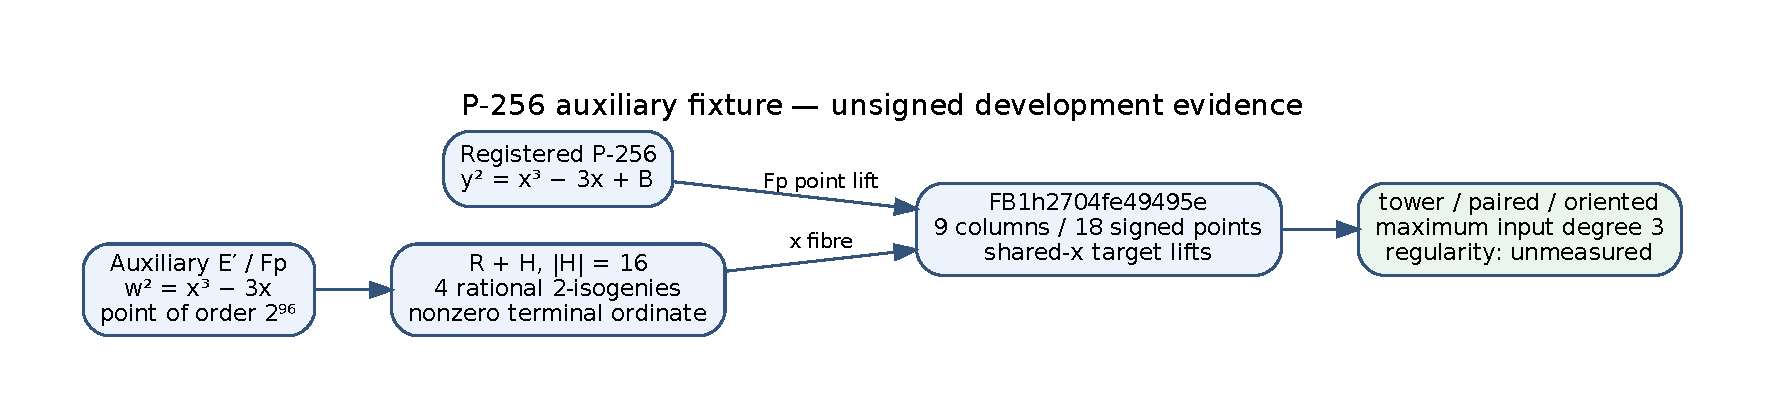
\includegraphics[width=\linewidth]{construction.pdf}

\textbf{Auxiliary construction.} Over the exact P-256 prime field,
$E':w^2=x^3-3x$ has proposed order $p+1$: since $p\equiv3\pmod4$,
the quadratic characters at $x$ and $-x$ cancel. The native certificate
checks a point of exact order $2^{96}$ with GMP/OpenSSL. Only that subgroup
is described as smooth. Choose $H$ of order 16, a rational 2-isogeny chain
$\phi$, and $R$ with $\phi(R)$ finite and not 2-torsion. Enumerate $R+H$,
then lift its distinct abscissae onto the target, retaining both signs.
The auxiliary slug is \texttt{icv1-fp256-t0-5593c5e9}.

\textbf{Presentations.} Each step has $\delta=3r^2+A\ne0$ and
\[
 (x_{i+1}-x_i)(x_i-r)-\delta=0,\qquad
 w_{i+1}(x_i-r)^2-w_i((x_i-r)^2-\delta)=0.
\]
Alignment gives $uv=B$, $u=y+w$, $v=y-w$. The paired arm has $2^m$
auxiliary-sign copies; fixing the terminal ordinate in the oriented arm
selects one per x but adds variables and equations. A win is not assumed.

\begin{center}
\begin{tabular}{rlrrr}
\toprule
$m$ & Arm & Input degree & Variables & Equations\\\midrule
2 & dense &9&13&44\\
2 & tower &3&19&50\\
2 & paired &3&23&54\\
2 & oriented &3&29&62\\\midrule
7 & dense &9&83&274\\
7 & tower &3&104&295\\
7 & paired &3&118&309\\
7 & oriented &3&139&337\\\bottomrule
\end{tabular}
\end{center}
Table: copied native export metadata, depth 4; unsigned and not a timing
comparison. All arms encode general addition, doubling, inverse and both
infinity-input cases. Comparisons are of $\mathbf F_p$-rational solutions,
not equal algebraic-closure ideals. Extension-valued outputs must be
rejected with their cost included. There is no target-log transport map.

\newpage
\textbf{Correctness evidence.} Complete depth 1 domains were compared for
$m=2\ldots7$, and depth 2 for $m=2\ldots4$, with planted and hash-selected
unplanted targets. Exhaustive and meet-in-the-middle ordered relation sets
matched in native tests. Every reported relation was replayed in GMP and
OpenSSL and evaluated in all four polynomial encodings. Forced exceptional
charts, reversed auxiliary ordinates and corrupted maps/orders/dumps were
also checked [pcc:unverified]. Small domains do not establish larger-base
natural yield or independence of collected rows.

\textbf{Executable CAS preparation.} The separate native Magma adapter
exports 48 programs ($m=2\ldots7$, two target kinds, four arms), sorted-name
grevlex order over the true 256-bit prime. It calls
\texttt{GroebnerBasis} then \texttt{Variety}. The reader projects actual
factor-base points, rejects malformed/truncated or incorrectly summed
relations, replays in exact group arithmetic and deduplicates projected
rows. Synthetic reader checks and static byte replay are unsigned evidence
under \texttt{PCC-20261114-91d75d}. \textbf{Magma itself was not executed.}
Its emitted affine output-basis degree must not be called regularity or
maximum F4 degree. A completion marker is not independent completeness proof.

\textbf{Original goal remains open.} Intended timing base depth 8 is not
replaced by this depth 4 development fixture. The owner's matched 2x
relation-stage target for every $m=2\ldots7$ still requires a qualified
complete CAS, exact input/source/image binding, warmup/A--A/five-round L2
panel, full costs and censored cells. Structured regularity needs its own
definition, homogenization and complete rank/degree evidence. Neither
novelty nor an end-to-end index-calculus improvement is asserted.

\textbf{Admission receipts.} Checkpoint upload gate exited 1 with no
configured transport. No EKS job or timed experiment was launched. The
current GitHub build bundle packages ecbench/fresh-owner, not this CAS
adapter. Root release-library validation could not start (cargo absent,
exit 127); this is not evidence of a root compiler defect. The precise
remaining gap is recorded in
\texttt{problems/p256-aligned-auxiliary-solver.md} [pcc:unverified].

\textbf{Reproduction.} In the study directory, use fresh output paths:
\begin{verbatim}
./run_checks.sh /tmp/aux-native-001
./run_adapter_checks.sh /tmp/aux-adapter-001
\end{verbatim}
Dependencies: C++20, GMP, OpenSSL, pkg-config, Bash and timeout.
Raw manifests, tests, compiler/dependency versions and source/binary hashes
are committed under \texttt{evidence/}. Failed compile001 is retained.
Read \texttt{PROTOCOL.md}, \texttt{REPORT.md} and \texttt{HANDOFF.md}
before launch; each prospective cell is capped at 60 seconds and 4 GiB,
single native process, without retries.

\textbf{Sources and prior art.}
Petit--Kosters--Messeng, PKC 2016, sections 3.1/3.4/3.5:
\href{https://people.maths.ox.ac.uk/petit/files/16PKC_primeECDLP.pdf}{primary paper}.
The framework and j=1728 auxiliary are prior art. Repository baseline source
pin is \texttt{0c2cc1b408e33a43e55ee31cb75307e90df9d619}; see
\texttt{prime\_tower.rs}, \texttt{p256\_dickson\_factor\_base.rs},
\texttt{curve\_id.rs} and \texttt{ecbench/canonical.rs}.
\href{https://magma.maths.usyd.edu.au/magma/handbook/text/1314}{Magma basis interface};
\href{https://magma.maths.usyd.edu.au/magma/handbook/text/1325}{rational variety interface}.
KB unavailable (no MCP tool; wrapper exit 127); fallback source review
does not establish novelty or absence. Existing performance dashboards
remain unchanged: there is no qualified new timing result.
\end{document}
